\documentclass{report}
 
\usepackage[ngerman]{babel}
\usepackage[utf8]{inputenc}
\usepackage[T1]{fontenc}
\usepackage{hyperref}
\usepackage{csquotes}
\usepackage{float}
\usepackage{caption}
\usepackage{graphicx}

\usepackage[
    backend=biber,
    style=authoryear,
    sortlocale=de_DE,
    natbib=true,
    url=false,
    doi=false,
    sortcites=true,
    sorting=nyt,
    isbn=false,
    hyperref=true,
    backref=false,
    giveninits=false,
    eprint=false]{biblatex}
\addbibresource{../references/bibliography.bib}


\title{Welche ethischen Herausforderungen entstehen durch den Einsatz von KI im Gesundheitswesen?}
\author{Lars}
\date{\today}


\parindent=0em


\begin{document}

\maketitle



\abstract{In diesem Dokument werden die Schwierigkeiten gschildert, die mit dem Einsatz von Künstlicher Intelligenz im Gsundheitswesen verbunden sind und welche ethischen Richtlinien es dabei zu beachten gilt.

}
    

\tableofcontents


\chapter{Einleitung}

\section{Was ist KI?}
Die Künstliche Intelligenz, geprägt von John McCarthy, umfasst Systeme, die menschliche Intelligenz mechanisch nachbilden. Dabei nutzt sie Sensoren zur Datenerfassung, Informationsverarbeitung zur Entscheidungsfindung und Aktoren zur Ausführung von Handlungen. 

\vspace{2mm}Die KI ist mittlerweile kaum mehr von unserer Gesellschaft wegzudenken. Dabei unterstützt sie uns beim Lösen komplexer Probleme. Was viele nicht wissen ist, dass es zwei Arten von KI gibt: schwache KI, die einfache Aufgaben erfüllen kann und diese auch mit wenigen Ausnahmen präzise ausführt, und die starke KI, die eine menschenähnliche Intelligenz und unabhängige Funktionsweisen aufweist und erfordert. Doch um eine starke KI zum Laufen zu bringen, muss sie erstmal die Funktionsweisen und Eigenschaften des menschlichen Geistes verstehen und in Systeme integriert werden, was ethische Herausforderungen aufwirft, insbesondere hinsichtlich der moralischen Behandlung solcher Systeme.

\vspace{2mm}Künstliche Intelligenz wird in sehr vielen Bereichen immer relevanter, so auch im Gesundheitswesen. Sie erlaubt präzisere Diagnosen und effizientere Behandlungen. Seit der COVID-19-Pandemie hat die Bedeutung von Technologien im Gesundheitswesen wie KI stark zugenommen.
\citep{ostfalia-de}

\vspace{25mm}

\section{Wie wird KI trainiert?}

Die künstliche Intelligenz hat das Potenzial, unser Leben stark zu verändern, sei es durch selbstfahrende Autos oder Roboter. Doch um diese Träume zu verwirklichen, muss das KI-System darauf trainiert werden.

\vspace{2mm}Es gibt drei Teilschritte beim Training unserer Assistenten (Training, Validierung und Testen). 

\vspace{2mm}Algorithmen werden im Trainingsprozess mit Daten gefüttert, dabei entstehen Vorhersagen und ihre Genauigkeit wird verbessert. Zum einen wird maschinell gelernt. Dabei lernen sie aus Daten und verbessern sich dabei fortlaufend. Zum anderen gibt es das Deep Learning. Es werden tiefe neuronale Netze eingesetzt, um gewisse Muster zu analysieren und zu erkennen.

\vspace{2mm}Zusätzlich gibt es auch noch weitere verschiedene Arten des Trainings, darunter überwachtes und unüberwachtes Lernen. Bei überwachtem Lernen werden gelabelte Daten verwendet, wodurch der Algorithmus wie beim maschinellen Lernen kontinuierlich trainiert wird. Also die KI lernt sich selbstständig. Im unüberwachten Lernen erkennt die KI, wie im Deep Learning, Muster, worin gelabelte Daten sind.

\vspace{2mm}Bei dem zweiten Schritt, der Validierung, wird die KI auf ihre Leistung mit neuen Daten geprüft. Das bringt das Ergebnis, ob das Modell verbessert werden muss oder das Training abgeschlossen ist.

\vspace{2mm}Schließlich im dritten Schritt, dem Testen, wird die gelernte KI in der realen Welt geprüft.

\citep{clickworker-de}


\begin{figure}[h]
    \centering 
    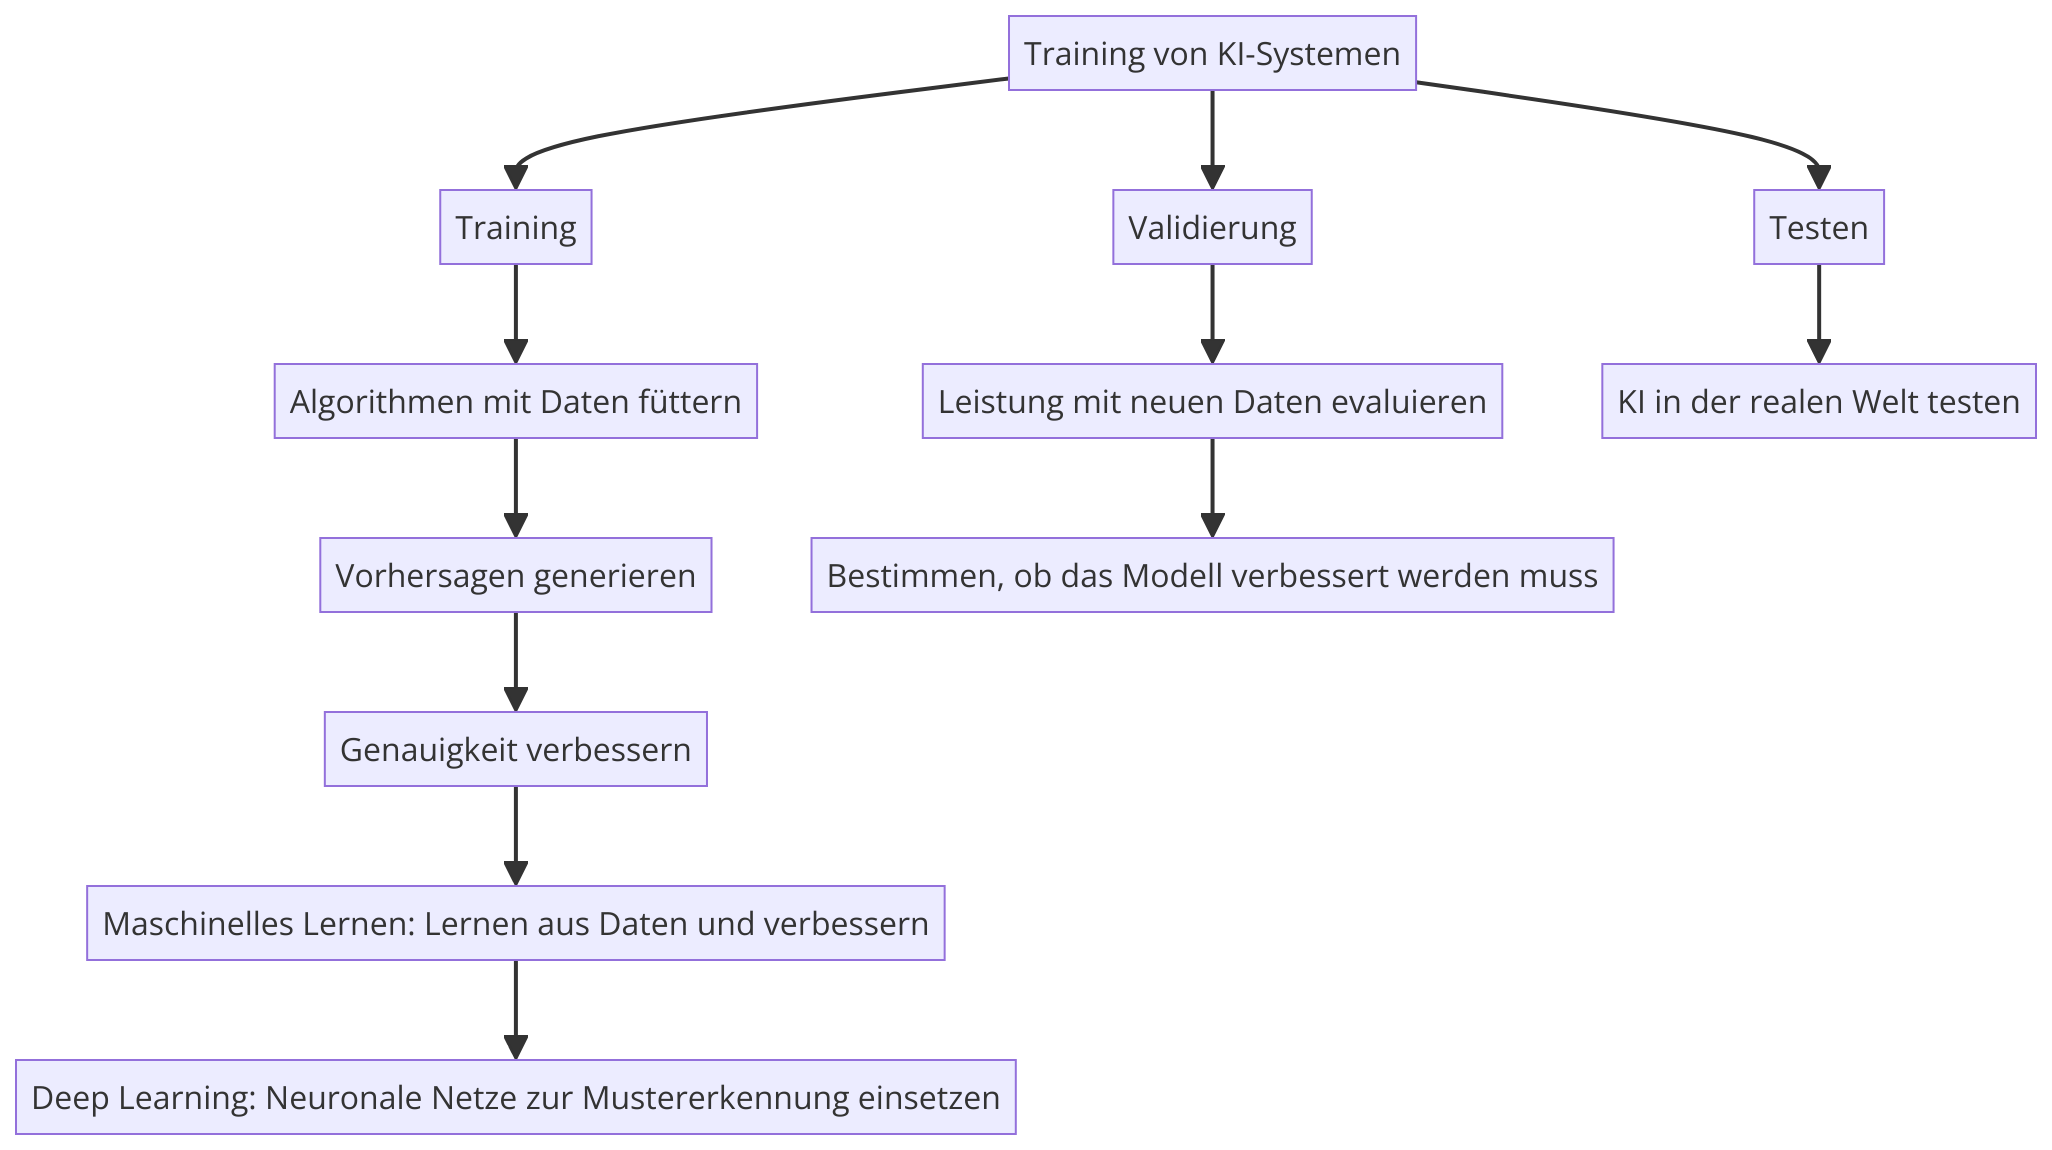
\includegraphics[width=0.8\textwidth]{diagram.png}
    \caption{3 Teilschritte beim Training einer KI}
    %\label{fig:meme}
    \end{figure}





\chapter{KI im Gesundheitswesen}

\section {Pro und Contras}
Die Einbindung von KI im Gesundheitswesen erfordert eine umfassende Beachtung von verschiedenen Faktoren, um einen nachhaltigen und erfolgreichen Einsatz zu gewährleisten.

\vspace{1mm}Die Künstliche Intelligenz bietet zahlreiche klinische Vorteile, wie präzise Diagnosen bis hin zu verbesserten Entscheidungsfindungen und noch besserer Überwachung der Patienten. Schlussendlich führt genau das zu einer schnelleren Versorgung der Patienten.

\vspace{1mm}Es können auch erhebliche Einsparungen im Gesundheitswesen ermöglicht werden, beispielsweise in der Früherkennung von Krankheiten, wodurch eine effizientere und schnellere Heilung ermöglicht wird. Dabei werden auch Kosten eingespart. Eine Studie belegt genau diese Kenntnis, dass durch den Einsatz von KI bei der Früherkennung von Erkrankungen wie Krebs und Demenz erheblich gespart werden kann, weil die Effizienz von Diagnose- und Behandlungsprozessen verbessert wird.

\vspace{6mm}Ein wichtiger Aspekt ist es, dass es starke Führungskräfte benötigt, die klare Visionen für den Einsatz von KI entwickeln können und in der Lage sind, agile Entscheidungen zu treffen. Diese Führungskräfte sollten nicht nur technologische Verständnisse haben und Innovationsbereitschaft mitbringen, sondern zusätzlich auch die Bedeutung von ethischen Richtlinien und Datenschutzbestimmungen betonen.

\vspace{1mm}Das Vertrauen in das Pflegepersonal, insbesondere der Ärzte, und in die KI-Technologie ist unerlässlich. Durch präzise Weiterbildungsmaßnahmen müssen die bestehenden Fähigkeiten an die neuen Anforderungen angepasst werden. Zum anderen ist es auch wichtig, die Patienten mit der KI-Nutzung während ihres Heilungsprozesses vertraut zu machen. Das Stoppen der Angst können Kommunikationskanäle ermöglichen, welche dabei positive und unbekannte Aspekte vermitteln sollen.Man sollte auch einen offenen Dialog über die Nutzung von KI mit der Bevölkerung führen. Nur so kann man das Vertrauen gewinnen und die Akzeptanz dazu fördern. Es ist wichtig, über die Potenziale und Grenzen von KI transparent zu informieren und den positiven Nutzen für die Patienten herauszustellen.

\vspace{25mm}Abschliessend kann man zusammenfassen, dass die verantwortungsvolle Nutzung der KI auch die Einhaltung von etishen Richtlinien erfordert. Damit die Privatsphäre und die Rechte der Betroffenen gewährt sind, müssen angemessene Regulierungen und robuste Datenschutzmaßnahmen gewährleistet sein. Dabei müssen Institutionen im Gesundheitswesen sicherstellen, dass die Anwendung ethisch vertretbar ist und den höchsten Standards in Bezug auf Sicherheit und Datenschutz entspricht.

\vspace{1mm}Eine ganzheitliche Herangehensweise, die diese zahlreichen Faktoren einbezieht, ist für die erfolgreiche Einbindung von KI im Gesundheitswesen von großer Bedeutung. Indem eine förderliche Unternehmenskultur geschaffen wird, das Vertrauen und die Fähigkeiten der Mitarbeiter gestärkt, der klinische und wirtschaftliche Nutzen verbessert, die gesellschaftliche Akzeptanz gefördert und ethische Standards sowie Datenschutzbestimmungen gewährleistet werden. Nur so kann KI zur Verbesserung der Gesundheitsversorgung und zur Steigerung der Effizienz des Gesundheitssystems beitragen.

\citep{pwc-de}







\printbibliography

\end{document}
